\chapter{Visualization}

\label{kap:visualization} % id kapitoly pre prikaz ref

To analyze the problems of different approaches we designed multiple visualizations.

\section{Raw data}

The simplest but often very helpful was to directly plot raw signals of all squiggles we were aligning. As all our approaches start with mean value and standard deviation preprocessing, 
we used these preprocessed data for visualization. We can see that this can reveal unexpected defects in data (Fig. \ref{fig:signals}). 

\begin{figure}[h]
  \centering
  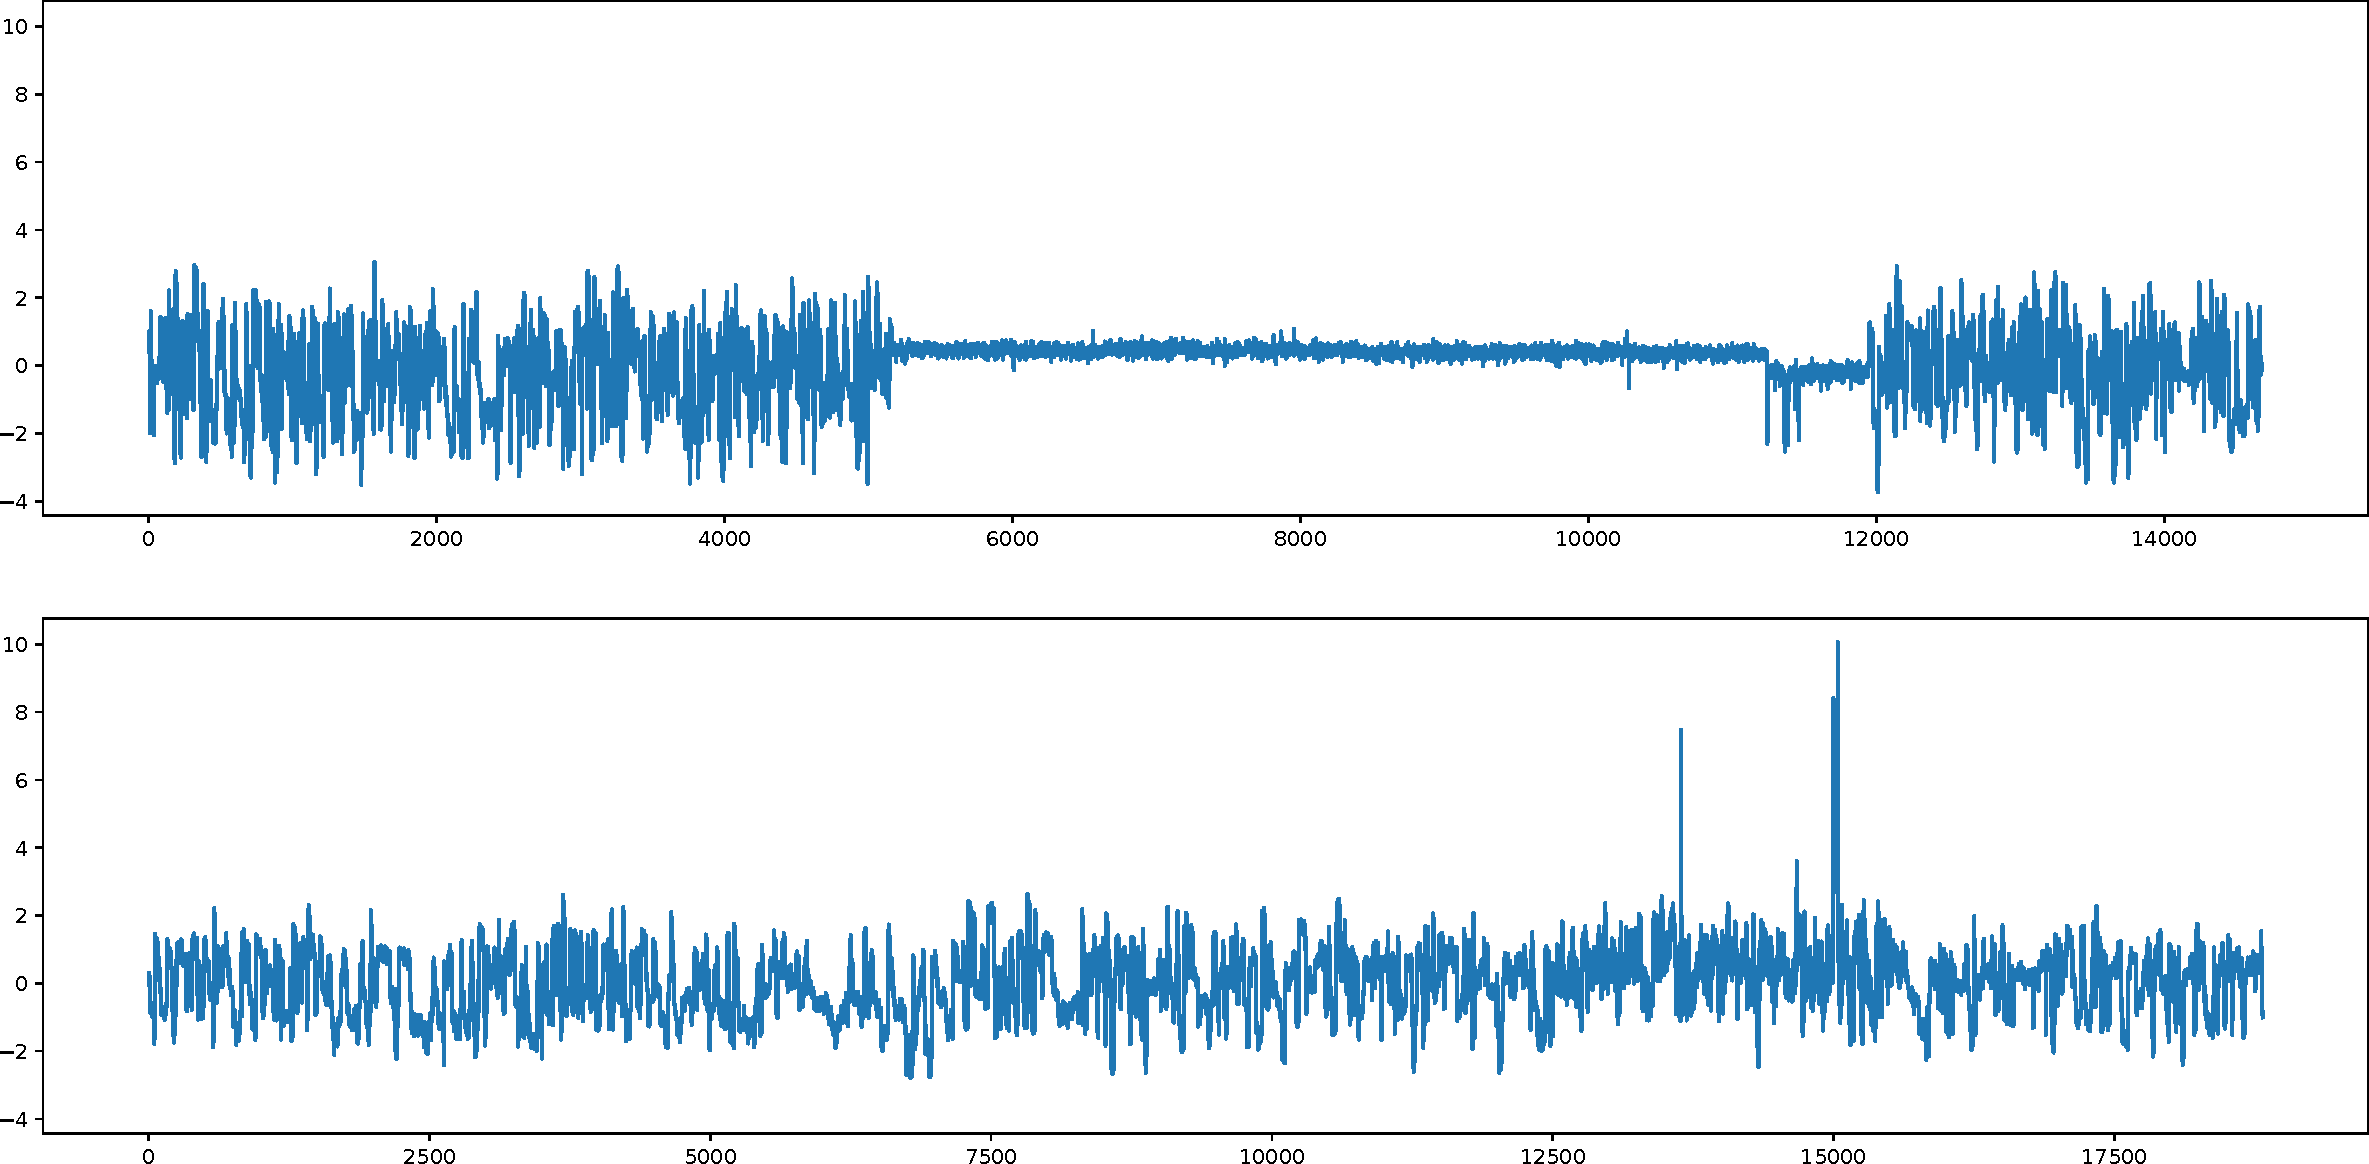
\includegraphics[width=1.0\textwidth]{images/signals}
  \caption{Defect data found by simple visualization.}
  \label{fig:signals}
\end{figure}

\section{Alignment}
To visualize single alignment of signals, we printed two signals vertically side by side and connected
aligned points between those plots (Fig. \ref{fig:pairing}). 

We also extended this visualization for progressive alignment. 
After each iteration of progressive alignment, we can generate the resulting signal and align it with the previous resulting signal to visualize
changes made by last added squiggle. This way we can plot all interim results underneath and print lines between successive pairs (Fig. \ref{fig:pairings}).

\begin{figure}[h]
  \centering
  \includegraphics[width=1.0\textwidth]{images/pairings}
  \caption{Insertions and deletions in process of progressive alignment.}
  \label{fig:pairings}
\end{figure}

To visualize all aligned squiggles in context of their consensus signal, we took the consensus signal as leading and aligned each squiggle to it.
This way we will loose omitted parts in squiggles, but all squiggles will have the same length and can be printed over each other with consensus signal (red) on top of them (Fig. \ref{fig:foos}).

\begin{figure}[h]
  \centering
  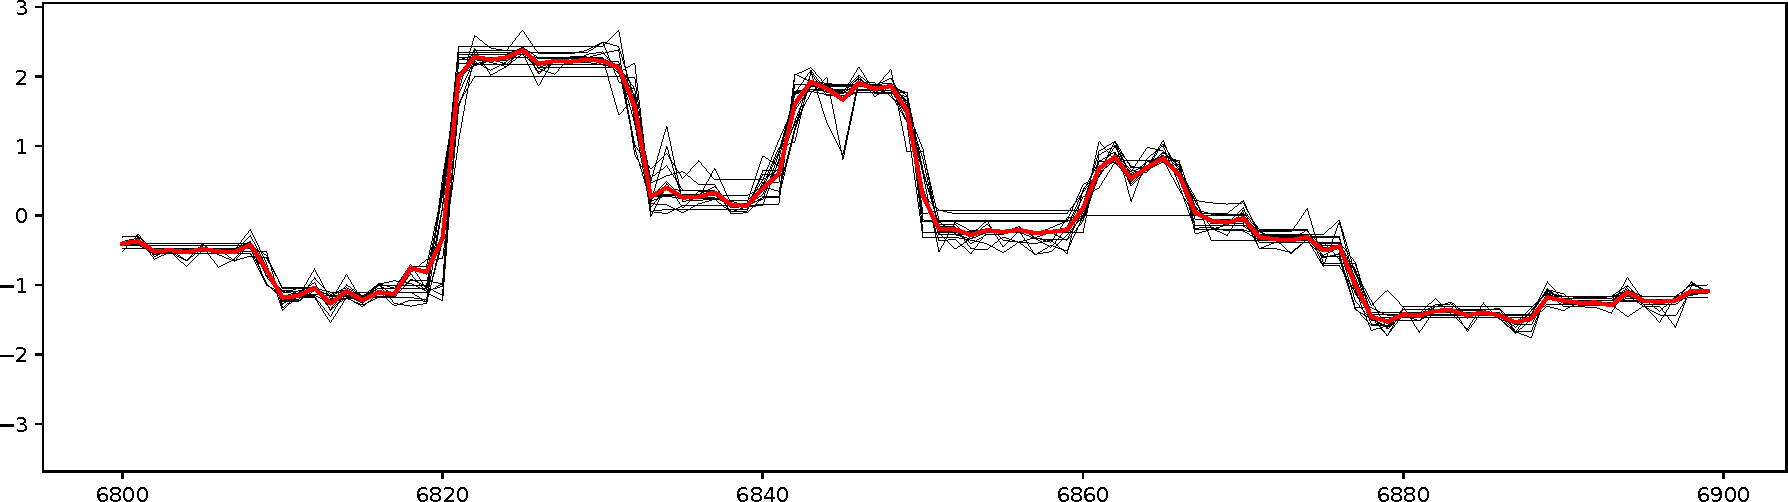
\includegraphics[width=1.0\textwidth]{images/foos}
  \caption{Aligned squiggles in context of consensus signal.}
  \label{fig:foos}
\end{figure}